% =============================================================================
% Bloque 4: Estado del Arte
% Intro SMOTE/ADASYN + Intro LLMs + Dilema + Timeline + Insights + Posicionamiento
% =============================================================================

\section{Estado del arte}

% --- Slide NUEVA (divulgación): qué es un embedding / el mapa de significados ---
% Imagen: Google ML Crash Course, "Embedding space" (CC BY 4.0), ejes traducidos.
\begin{frame}{La pieza clave: convertir cada texto en un punto de un mapa}
\begin{columns}[T]

\begin{column}{0.44\textwidth}
\small
Los computadores no leen palabras: leen \textbf{números}.

\vspace{0.4em}
Un modelo de \textbf{embeddings} le hace muchas preguntas a cada texto y lo convierte en \textbf{un punto de un mapa}.

\vspace{0.4em}
\textbf{La propiedad clave:}
\begin{itemize}\setlength\itemsep{2pt}
  \item Cosas con significado \alert{parecido} quedan \alert{cerca}.
  \item Las que no tienen nada que ver quedan lejos.
\end{itemize}

\vspace{0.4em}
{\footnotesize Todo lo que viene ocurre en ese mapa: cada oración, real o inventada, es \textbf{un punto}.}
\end{column}

\begin{column}{0.54\textwidth}
\centering
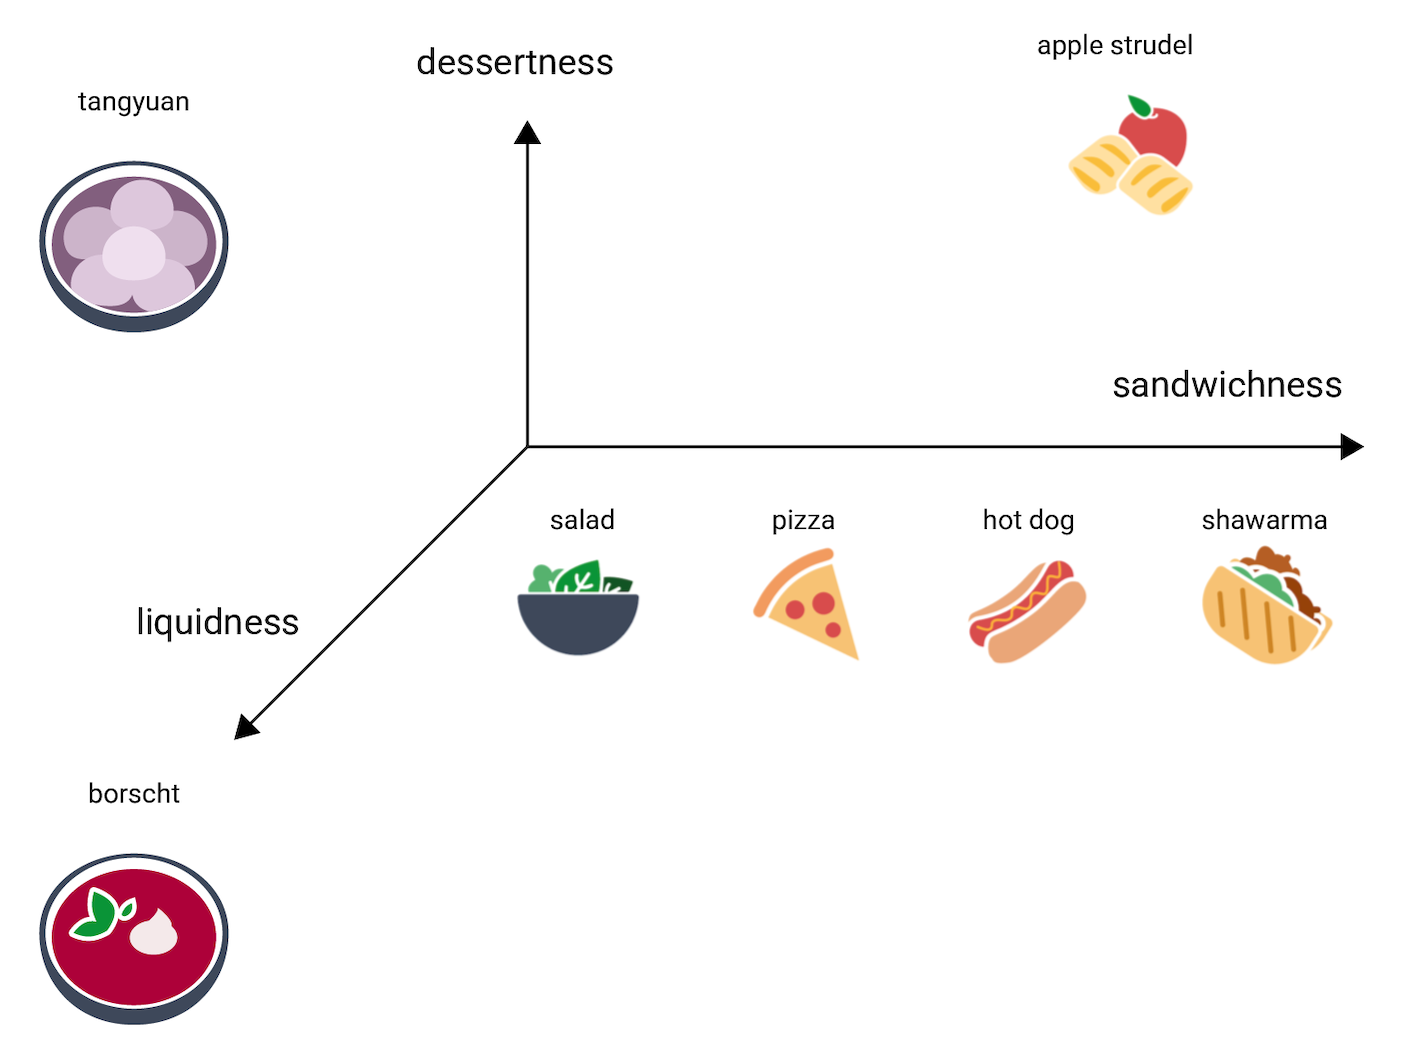
\includegraphics[height=4.6cm]{embeddings_3D_tangyuan.png}\\[1pt]
{\scriptsize\itshape Con comidas bastan 3 preguntas. Con texto es igual, pero con \textbf{cientos}.}\\[1pt]
{\tiny\color{uaigray} Imagen de Google, \textit{ML Crash Course} (CC BY 4.0).}
\end{column}

\end{columns}

\mensaje{Con los textos convertidos en puntos, «parecerse» se vuelve algo que podemos \emph{medir}.}
\end{frame}

% --- Slide: Intro SMOTE (simplificada para divulgación; fórmula fuera) ---
\begin{frame}{Camino 1 — SMOTE: inventar puntos intermedios en el mapa}
\begin{columns}[T]

\begin{column}{0.55\textwidth}
\small
\textbf{SMOTE} \cita{Chawla et al., 2002} es el método clásico (20+ años) para crear ejemplos de la clase escasa.

\vspace{0.4em}
\textbf{La idea, en una frase:}
\begin{itemize}\setlength\itemsep{2pt}
  \item Toma dos ejemplos reales que sean vecinos en el mapa\dots
  \item \dots{}y crea un punto nuevo \alert{en el camino entre ambos}: un «promedio» de los dos.
\end{itemize}

\vspace{0.6em}
\good\ Controlado: nunca se sale de la zona conocida.\\
\good\ Simple y rápido; funciona hace décadas.\\[3pt]
\bad\ Genera \alert{puntos, no texto}: no hay oración nueva que leer.\\
\bad\ Solo \alert{rellena} lo que ya se sabe: no aporta variedad nueva.
\end{column}

\begin{column}{0.45\textwidth}
\centering
\vspace{0.3em}
\begin{tikzpicture}[scale=1.0]
  % Casco convexo
  \fill[methodSMOTE!10] (-1.3,-1.1) -- (1.3,-0.9) -- (1.5,0.7) -- (-0.5,1.3) -- (-1.3,-1.1);

  % Puntos reales
  \foreach \pt in {(-1.3,-1.1),(1.3,-0.9),(1.5,0.7),(-0.5,1.3),(0,0.2)}{\fill[methodSMOTE] \pt circle (3.5pt);}

  % Segmentos de interpolación
  \draw[methodSMOTE!60, dashed] (-1.3,-1.1) -- (1.3,-0.9);
  \draw[methodSMOTE!60, dashed] (-1.3,-1.1) -- (0,0.2);
  \draw[methodSMOTE!60, dashed] (0,0.2) -- (1.5,0.7);
  \draw[methodSMOTE!60, dashed] (-0.5,1.3) -- (0,0.2);

  % Sintéticos (en los segmentos)
  \foreach \pt in {(0,-1),(-0.65,-0.45),(0.75,0.45),(-0.25,0.75)}{\draw[uaiorange, very thick] \pt circle (3pt);}

  \node[font=\tiny, color=uaigray] at (0,-1.8) {{\color{methodSMOTE}\textbullet}\,reales \quad {\color{uaiorange}$\circ$}\,inventados};
  \node[font=\tiny\itshape] at (0,-2.1) {Puntos nuevos entre vecinos};
\end{tikzpicture}
\end{column}

\end{columns}

\mensaje{Control total sobre dónde caen los puntos\dots\ pero sin texto nuevo y sin nada realmente nuevo.}
\end{frame}

% =============================================================================
% [DIVULGACIÓN] Slide comentada para la versión de público general.
% Reactivar quitando \iffalse ... \fi si se necesita de nuevo (versión defensa).
% =============================================================================
\iffalse
% --- Slide: Familia 2 — Aumentación textual ligera (entre SMOTE y LLMs) ---
\begin{frame}{Familia 2 — Aumentación textual ligera}
\small
Entre la \alert{interpolación geométrica} y la \alert{generación libre} hay un puente histórico: métodos que producen texto con modelos pequeños y operaciones controladas.

\vspace{0.5em}
\begin{columns}[T]

\begin{column}{0.33\textwidth}
\setbeamercolor{block title}{fg=white,bg=uaiblue}
\begin{block}{EDA}
\scriptsize
\cita{Wei \& Zou, 2019}\\[3pt]
4 ops a nivel \textbf{palabra}:\\
sinónimo, inserción, swap, deleción.\\[3pt]
\good\ Muy barato.\\
\bad\ Ruido en oraciones cortas.
\end{block}
\end{column}

\begin{column}{0.33\textwidth}
\setbeamercolor{block title}{fg=white,bg=uaiblue}
\begin{block}{Traducción inversa}
\scriptsize
\cita{Sennrich 2016; Edunov 2018}\\[3pt]
EN $\to$ otro idioma $\to$ EN.\\
Paráfrasis a nivel \textbf{oración}.\\[3pt]
\good\ Cambia sintaxis.\\
\bad\ Pierde matices.
\end{block}
\end{column}

\begin{column}{0.33\textwidth}
\setbeamercolor{block title}{fg=white,bg=uaiblue}
\begin{block}{BERT contextual}
\scriptsize
\cita{Kobayashi 2018; Wu 2019}\\[3pt]
Enmascarar tokens; BERT predice alternativas plausibles.\\[3pt]
\good\ Contexto semántico.\\
\bad\ Solo sustitución 1:1.
\end{block}
\end{column}

\end{columns}

\vspace{0.7em}
\begin{insight}
\scriptsize
Todos producen \textbf{texto}, pero con un \textbf{techo de creatividad bajo}: paráfrasis cercanas al original. Los LLMs rompen ese techo --- y por eso necesitan otro tipo de control.
\end{insight}
\end{frame}
\fi

% --- Slide: Camino 2 — LLMs ---
\begin{frame}{Camino 2 — Pedirle los ejemplos a una IA (LLM)}
\begin{columns}[T]

\begin{column}{0.58\textwidth}
\small
Pedirle a una IA generativa (ChatGPT, Gemini, Claude\dots) que \textbf{escriba ejemplos nuevos} para la clase que tiene pocos.

\vspace{0.4em}
\textbf{La receta que se usa hoy:}
\begin{enumerate}\setlength\itemsep{2pt}\small
  \item Mostrarle los pocos ejemplos reales que hay.
  \item Pedirle: «escribe 50 más como estos».
  \item Agregar \textbf{todo} lo que responda al entrenamiento.
\end{enumerate}

\vspace{0.4em}
Varios estudios reportan mejoras \cita{Whitehouse 2023; Suhaeni 2024; Cegin 2025} — pero todos comparten el mismo punto ciego.

\vspace{0.4em}
{\small
\good\ Texto real, fluido y variado.\\
\bad\ \alert{Nadie revisa dónde caen} esos textos en el mapa: se acepta todo, bueno y malo.}
\end{column}

\begin{column}{0.42\textwidth}
\centering
\vspace{0.2em}
\begin{tikzpicture}[every node/.style={font=\scriptsize, align=center}]
  \node[draw=uaibluedark, fill=uaibluelight!15, rounded corners, very thick,
        text width=3.6cm, minimum height=1.0cm] (prompt) at (0, 2.7)
        {\scriptsize\textbf{Prompt}\\[1pt]
         \tiny\itshape ``Genera 50 mensajes de alegría\dots''};
  \draw[->, very thick, uaibluedark] (0, 2.05) -- (0, 1.65);
  \node[draw=methodOurs, fill=methodOurs!15, rounded corners, very thick,
        text width=2.4cm, minimum height=0.7cm] (llm) at (0, 1.2)
        {\textbf{LLM}};
  \draw[->, very thick, methodOurs] (0, 0.8) -- (0, 0.4);
  \node[draw=uaiorange, fill=uaiorange!10, rounded corners, very thick,
        text width=3.6cm, minimum height=1.0cm] (out) at (0, -0.2)
        {\scriptsize\textbf{$N$ oraciones nuevas}\\[1pt]
         \tiny algunas buenas, otras ruido\dots};
\end{tikzpicture}
\end{column}

\end{columns}

\mensaje{Texto rico pero sin control: los puntos caen donde quieran en el mapa.}
\end{frame}

% =============================================================================
% [DIVULGACIÓN] Slide comentada para la versión de público general.
% Reactivar quitando \iffalse ... \fi si se necesita de nuevo (versión defensa).
% =============================================================================
\iffalse
% --- Slide: Familia 3.5 — Fine-tuning para generación sintética ---
\begin{frame}{Familia 3.5 — \textit{Fine-tuning} para generación sintética}
\begin{columns}[T]

\begin{column}{0.58\textwidth}
\small
Una rama más reciente: \alert{ajustar el LLM} sobre la propia tarea antes de generar.

\vspace{0.2em}
\textbf{Idea:} fine-tunear un LLM preentrenado (GPT-2, LLaMA, T5\dots) con los pocos ejemplos disponibles, y luego generar muestras \emph{específicas} del dominio.

\vspace{0.3em}
\textbf{Trabajos representativos:}
\begin{itemize}\setlength\itemsep{0pt}\scriptsize
  \item Cloutier \& Japkowicz (2023): \alert{fine-tuning generativo} supera al re-muestreo tradicional en multiclase desbalanceada.
  \item ImbLLM (Nguyen et al., 2024): fine-tuning \textbf{solo en muestras minoritarias}; F1\,$>$\,0.8.
  \item SentiGEN (Sundararajan, 2023): T5 fine-tuned + validador XLNet.
\end{itemize}

\vspace{0.3em}
{\scriptsize
\good\ Distribución alineada con la tarea.\\
\bad\ Requiere \alert{cómputo extra}; riesgo de \emph{overfitting} con $n$ pequeño.}
\end{column}

\begin{column}{0.42\textwidth}
\centering
\vspace{0.1em}
\begin{tikzpicture}[every node/.style={font=\scriptsize, align=center}, scale=0.92, transform shape]
  % LLM base
  \node[draw=uaibluedark, fill=uaibluelight!15, rounded corners, very thick,
        text width=3.0cm, minimum height=0.55cm] (base) at (0, 2.6)
        {\textbf{LLM preentrenado}\\\tiny GPT-2, LLaMA, T5\dots};

  % Few-shot data
  \node[draw=methodSMOTE, fill=methodSMOTE!15, rounded corners, very thick,
        text width=1.9cm, minimum height=0.45cm, font=\scriptsize] (data) at (-1.95, 1.55)
        {Pocos ej.};

  % Fine-tune arrow
  \node[draw=uaiamber, fill=uaiamber!15, rounded corners, very thick,
        text width=1.7cm, minimum height=0.45cm, font=\scriptsize\bfseries] (ft) at (0.6, 1.55)
        {Fine-tuning};
  \draw[->, very thick, uaiamber] (data) -- (ft);
  \draw[->, very thick, uaiamber] (base) -- (ft);

  % LLM ajustado
  \node[draw=methodOurs, fill=methodOurs!15, rounded corners, very thick,
        text width=3.0cm, minimum height=0.55cm] (llmft) at (0, 0.55)
        {\textbf{LLM ajustado}\\\tiny especializado};
  \draw[->, very thick, methodOurs] (ft) -- (llmft);

  % Output
  \node[draw=uaiorange, fill=uaiorange!10, rounded corners, very thick,
        text width=3.0cm, minimum height=0.5cm] (out) at (0, -0.45)
        {\scriptsize\textbf{Muestras sintéticas}\\\tiny alineadas al dominio};
  \draw[->, very thick, uaiorange] (llmft) -- (out);
\end{tikzpicture}
\end{column}

\end{columns}

\mensaje{Más alineamiento, más costo: distinto eje de control al filtrado posterior.}
\end{frame}
\fi

% --- Slide: El dilema (movido desde Introducción) ---
\begin{frame}{El dilema: SMOTE vs.\ LLMs lado a lado}
\begin{columns}[T]

\begin{column}{0.5\textwidth}
\centering
\setbeamercolor{block title}{fg=white,bg=methodSMOTE}
\begin{block}{SMOTE / interpolación}
\small
\good\ Sabemos \textbf{dónde} caen sus puntos\\
\good\ Probado por más de 20 años\\[2pt]
\bad\ No produce texto nuevo\\
\bad\ Solo rellena lo ya conocido
\end{block}
\vspace{0.2em}
\begin{tikzpicture}[scale=0.85]
  \fill[methodSMOTE!20] (0,0) circle (1.4);
  \foreach \pt in {(0,0.4),(0.7,0.2),(-0.5,0.6),(0.3,-0.5),(-0.7,-0.3),(0.6,-0.7)} {\fill[methodSMOTE] \pt circle (2pt);}
  \foreach \pt in {(0.4,0),(-0.2,0.1),(0.1,0.5),(-0.4,-0.5),(0.45,-0.2)} {\draw[uaiorange,thick] \pt circle (2pt);}
  \node[font=\tiny] at (0,-1.7) {Todo queda dentro de la zona conocida};
\end{tikzpicture}
\end{column}

\begin{column}{0.5\textwidth}
\centering
\setbeamercolor{block title}{fg=white,bg=methodOurs}
\begin{block}{LLM (Gemini, GPT, Claude\dots)}
\small
\good\ Texto fluido y variado\\
\good\ Aporta contenido \textbf{nuevo}\\[2pt]
\bad\ No sabemos dónde caen sus puntos\\
\bad\ Puede mezclar clases (ruido)
\end{block}
\vspace{0.4em}
\begin{tikzpicture}[scale=0.85]
  \fill[methodOurs!15] (0,0) circle (1.6);
  \foreach \pt in {(0,0.4),(0.7,0.2),(-0.5,0.6),(0.3,-0.5)} {\fill[methodOurs] \pt circle (2pt);}
  \foreach \pt in {(0.4,0),(-0.2,0.1),(0.1,0.5),(1.4,0.3),(-1.2,-0.4),(0.9,-1.0),(-0.8,1.1)} {\draw[uaiorange,thick] \pt circle (2pt);}
  \node[font=\tiny] at (0,-1.9) {Los puntos caen donde sea};
\end{tikzpicture}
\end{column}

\end{columns}

\mensaje{¿Podemos quedarnos con lo mejor de ambos mundos?}
\end{frame}

% =============================================================================
% [DIVULGACIÓN] Slide comentada para la versión de público general.
% Reactivar quitando \iffalse ... \fi.
% =============================================================================
\iffalse
% --- Slide: Tres deficiencias (después del Timeline) ---
\begin{frame}{Tres deficiencias en los métodos actuales}
\small
\begin{columns}[T]

\begin{column}{0.33\textwidth}
\setbeamercolor{block title}{fg=white,bg=uaiorange}
\begin{block}{1. Sin control de calidad}
Lo que escribe la IA se acepta \textbf{todo}, sin revisar si cada texto cayó en la zona correcta del mapa.
\vspace{0.3em}\\
{\scriptsize Que esté bien escrito $\neq$ que sea un buen ejemplo.}
\end{block}
\end{column}

\begin{column}{0.33\textwidth}
\setbeamercolor{block title}{fg=white,bg=uaiamber}
\begin{block}{2. Todo pesa igual}
Al entrenar, un ejemplo dudoso cuenta \textbf{lo mismo} que uno excelente.
\vspace{0.3em}\\
{\scriptsize Nadie distingue entre buenos y mediocres.}
\end{block}
\end{column}

\begin{column}{0.33\textwidth}
\setbeamercolor{block title}{fg=white,bg=uaiblue}
\begin{block}{3. Poca evidencia}
Casi todos los estudios prueban su método en \textbf{un solo} conjunto de datos.
\vspace{0.3em}\\
{\scriptsize ¿Funcionará también en otros temas y tareas?}
\end{block}
\end{column}

\end{columns}

\vfill
\begin{tikzpicture}[overlay,remember picture]
\end{tikzpicture}

\mensaje{El mapa ya existe y nadie lo está usando para controlar la calidad.}
\end{frame}
\fi

% --- Slide: Gap metodológico + idea conceptual ---
\begin{frame}{La idea de esta tesis: ponerle un control de calidad a la IA}
\begin{columns}[T]

\begin{column}{0.52\textwidth}
\small
Nadie revisa dónde caen los textos que escribe la IA. Eso abre una solución sorprendentemente simple.

\vspace{0.2em}
\textbf{La idea:}
\begin{enumerate}\setlength\itemsep{1pt}\footnotesize
  \item Pedirle a la IA \textbf{más ejemplos de los necesarios}.
  \item Ubicar cada uno como un punto en el mapa.
  \item Medir qué tan cerca cae de los \textbf{ejemplos reales} de su clase.
  \item \alert{Descartar los que caen demasiado lejos}.
\end{enumerate}

\vspace{0.3em}
\textbf{¿Por qué tiene sentido?}
\begin{itemize}\setlength\itemsep{1pt}\footnotesize
  \item El mapa \alert{ya lo teníamos}: es el mismo que usa el clasificador.
  \item Sirve cualquier IA (Gemini, GPT, Claude\dots): no hay que abrirla ni re-entrenarla.
\end{itemize}
\end{column}

\begin{column}{0.48\textwidth}
\centering
\vspace{0.2em}
\begin{tikzpicture}[scale=0.85]
  % Cluster real (fondo)
  \fill[methodSMOTE!18] (0,0) circle (1.5);

  % Frontera del filtro (dashed)
  \draw[uaibluedark, dashed, thick] (0,0) circle (1.9);

  % Puntos reales (sólidos)
  \foreach \pt in {(0,0.2),(0.4,0.4),(-0.5,0.3),(0.6,-0.4),(-0.3,-0.5),(0.2,0.7),(-0.6,-0.2),(0.7,0.1)} {\fill[methodSMOTE] \pt circle (3pt);}

  % LLM aceptados (verdes, dentro del filtro)
  \foreach \pt in {(0.9,0.5),(-0.8,-0.7),(0.3,1.0),(-0.4,1.1),(1.0,-0.5),(-1.1,0.4)} {\draw[methodOurs, very thick] \pt circle (3pt);}

  % LLM rechazados (rojos, fuera del filtro)
  \foreach \pt in {(2.4,0.7),(-2.3,0.9),(2.0,-1.4),(-1.7,-2.0),(0.1,2.3),(2.5,-0.3)} {\draw[uaiorange, very thick] \pt circle (3pt);}

  % Leyenda compacta
  \node[font=\tiny, color=methodSMOTE, anchor=west] at (-2.8,3.0) {{\fontsize{6}{6}\selectfont$\bullet$}\,reales};
  \node[font=\tiny, color=methodOurs, anchor=west] at (-2.8,2.7) {$\circ$\,aceptado};
  \node[font=\tiny, color=uaiorange, anchor=west] at (-2.8,2.4) {$\circ$\,rechazado};
  \node[font=\tiny, color=uaibluedark, anchor=west] at (-2.8,2.1) {- -\,filtro};
\end{tikzpicture}
\end{column}

\end{columns}

\mensaje{Lo mejor de ambos mundos: el texto lo pone la IA, el control de calidad lo pone el mapa.}
\end{frame}

